\documentclass[a4paper,10pt]{article}

\usepackage[boxruled,vlined,english]{algorithm2e}
\usepackage[francais,english]{babel}
\usepackage[utf8x]{inputenc}
\usepackage[T1]{fontenc}
\usepackage{graphicx}
\usepackage{hyperref}
\usepackage{latexsym}
\usepackage{setspace}
\usepackage{amsmath}
\usepackage{amssymb}
\usepackage{bookman}
\usepackage{amsthm}
\usepackage{amscd}
\usepackage{color}
\usepackage{calc}

\setlength{\voffset}{-3.75cm}
\setlength{\hoffset}{-2.6cm}
\setlength{\oddsidemargin}{2.75cm}
\setlength{\topmargin}{2in}
\setlength{\headheight}{0in}
\setlength{\headsep}{0in}
\setlength{\topskip}{0in}
\setlength{\parindent}{0cm}
\setlength{\parskip}{1ex plus0.4ex minus0.2ex}
\setlength{\textwidth}{16.25cm}
\setlength{\textheight}{21cm}
\renewcommand{\baselinestretch}{1.5}
\flushbottom
\setcounter{page}{1}
\setcounter{tocdepth}{2}

\SetKw{Edb}{Side effect}
\SetKw{Et}{and}
\SetKw{Ou}{or}
\SetKw{De}{from}
\SetKw{A}{to}
\SetKw{Par}{by}
\SetKwBlock{Debut}{Begin}{End}
\SetKwIF{Si}{SinonSi}{Sinon}{If}{then}{Else if}{Else}{EndIf}
\SetKwFor{Pour}{For}{do}{EndFor}
\SetKwFor{PourTout}{For all}{do}{EndFor}
\SetKwFor{TantQue}{While}{do}{EndWhile}
\SetKw{Retour}{Return}

\newcommand{\guill}[1]{``#1''}
\newcommand{\bigO}[1]{\mathcal O\left( #1 \right)}
\newcommand{\bigOmega}[1]{\Omega\left( #1 \right)}
\newcommand{\bigTheta}[1]{\Theta\left( #1 \right)}

\newtheorem{prob}{Problem}


% ??? Faire une Titlepage un peu plus jolie...
\title{ \Large Appendix \\ \LARGE Computational analysis of jazz chord sequences}

\author{\normalsize Romain \textsc{Versaevel}, M1 Informatique Fondamentale, ENS de Lyon \\ \normalsize Tutored by David \textsc{Meredith}, Associate professor at Aalborg University\\}

\date{\today}

\begin{document}

\maketitle
%\newpage
\tableofcontents
\newpage


\section{List and definitions of all similarity measures}

\subsubsection*{Equality, root notes, translation}

Let us consider two chords $C_1 = R_1 H_1$ and $C_2 = R_2 H_2$, where $R_i$ denotes the root note and $H_i$ the harmonic label.
The first three similarity measures are then defined by:

\begin{equation*}
\mathfrak{M}_{root}(C_1,C_2) = 1 \Leftrightarrow R_1 = R_2
\end{equation*}

\begin{equation*}
\mathfrak{M}_{translation}(C_1,C_2) = 1 \Leftrightarrow H_1 = H_2
\end{equation*}

\begin{align*}
\mathfrak{M}_{eq}(C_1,C_2) = 1 & \Leftrightarrow C_1 = C_2 \\
& \Leftrightarrow \mathfrak{M}_{root}(C_1,C_2) = \mathfrak{M}_{translation}(C_1,C_2) = 1
\end{align*}


\subsubsection*{PCS-prime equivalence}

Formally, $\mathfrak{M}_{PCS}(C_1,C_2) = 1$ if and only if $C_1$ can be obtained from $C_2$ by combining the following two operations:

\begin{align*}
\text{translation} :~& \mathcal{P}([0,12])\times\mathbb{N} \longrightarrow \mathcal{P}([0,12]) \\
 & (\{x_i\}_i, t) \longmapsto \{(x_i+t)\mod 12\}_i \\
\text{inversion} :~& \mathcal{P}([0,12]) \longrightarrow \mathcal{P}([0,12]) \\
 & \{x_i\}_i \longmapsto \{(12-x_i)\}_i
\end{align*}

The algorithmical way to compute $\mathfrak{M}_{PCS}(C_1,C_2)$ is a bit technical but an excellent description can be found on \href{http://composertools.com/Theory/PCSets.pdf}{http://composertools.com/Theory/PCSets.pdf}.


\subsubsection*{Morris', Rahn's, Lewin's, Teitelbaum's and Isaacson's measures}

All the following measures imply the use of \emph{interval vectors}, as defined in the main report. Hence, let us now for more clarity call the two chords to compare $X$ and $Y$. Their interval vectors are $IV_X=(x_1,\dots,x_6)$ and $IV_Y=(y_1,\dots,y_6)$. We also define $D(X,Y)$, the difference vector $((y_1-x_1),\dots,(y_6-x_6))$.

Morris' measure is the sum of absolute values of the coordinates of $D$:

\begin{align*}
\mathfrak{M}_{Morris}(X,Y)& = \sum_{i=1}^6 \left|D(X,Y)\right|& = \sum_{i=1}^6 \left|y_i-x_i\right|
\end{align*}

Rahn's measure sums the entries of the interval vectors of $X$ and $Y$, but only for the coordinates $i$ such that both $IV(X)_i$ and $IV(Y)_i$ are non-zero (if for instance $X$ has intervals of length $4$ but $Y$ does not, these are not taken into account). It is then scaled in order to get values in $[0,1]$:


\begin{align*}
\mathfrak{M}_{Rahn}(X,Y) = \sum_{i=1}^6 \left[\left(IV(X)_i+IV(Y)_i\right)\cdot\textbf{1}_{IV(X)_i\geq1\text{ and }IV(Y)_i\geq1}\right] \cdot \frac{2}{|X|(|X|-1)+|Y|(|Y|-1)}
\end{align*}

Lewin's measure consists in the sum of the square roots of products of the coordinates of $IV(X)$ and $IV(Y)$ (like in Rahn's, a single coordinate is equal to $0$ leads to a zero term). It is also properly scales:

\begin{align*}
\mathfrak{M}_{Lewin}(X,Y) = \sum_{i=1}^6 \left[\sqrt{IV(X)_i\cdot IV(Y)_i}\right] \cdot \frac{2}{\sqrt{|X|(|X|-1)|Y|(|Y|-1)}}
\end{align*}

Teitelbaum's measure is the euclidean distance applied on the interval vectors:

\begin{align*}
\mathfrak{M}_{Teitebaum}(X,Y) = \sqrt{\sum_{i=1}^6 \left[(IV(X)_i-IV(Y)_i)^2\right]}
\end{align*}

Finally, and as described in the main report, Isaacson's similarity index is the standard deviation function applied to the interval vectors. If $\bar{D}$ denotes the mean of the $(y_i-x_i)$s, it is:

\begin{equation*}
\mathfrak{M}_{Isaacson}(X,Y) = \sqrt{\frac{1}{6}\left(\sum_{i=1}^6\left(D_i-\bar{D}\right)^2\right)}
\end{equation*}

\subsubsection*{Similarity of sequences}

%For all measures, two chord sequences $(C_i)_{1\leq i\leq n}$ and $(C_'i)_{1\leq i\leq n}$ of the same length $n$ will be considered similar according to a certain threshold $t$ if $\forall 0\leq i\leq n, \mathfrak{M}(C_i,C'_i) \geq t$\footnote{I did keep the definitions from the original papers, so no homogenization has been made, and for some a better similarity means being closer to $0$, so it would be $\leq$ instead of $\geq$}.

The only exception is $\mathfrak{M}_{translation}$, which allows a more precise extension to sequences: the \emph{difference} (in the mapping to $\mathbb{Z}/12\mathbb{Z}$) between corresponding notes should all be the same: $\exists d \in \mathbb{Z}/12\mathbb{Z}, \forall 0\leq i\leq n, \mathfrak{M}_{translation}(C_i,C'_i) = true \wedge (C'_i-C_i)\mod12 = d$.

For instance, if we consider the sequences:

\begin{center}
\begin{tabular}{l}
$S = Am;~B;~G7;~A$ \\
$S' = Dm;~E;~C7;~D$ \\
$S'' = Am;~E;~F7;~B$ \\
$S''' = A9;~E;~FM7;~B7\flat5$ \\
\end{tabular}
\end{center}

$S$ and $S'$ are similar ($d=-7\mod12=5$), but $S$ and $S''$ are not (the difference between $A$ and $A$ is $0$, and $-7\mod12=5$ between $B$ and E); and sequences $S''$ and $S'''$ are dissimilar because despite a constant difference ($0$) between root notes, the harmonic labels are different.

\newpage

\section{LZ77: a full example example}

Here I give an example of an execution of the LZ77 algorithm (without restriction on the buffer and preview sizes). The algorithm pseudo-code is recalled in algorithm \ref{algolz77}.

\begin{algorithm}
\setstretch{1.5}
\caption{LZ77 \label{algolz77}}
\SetKwData{jjj}{j} \SetKwData{III}{I} \SetKwData{nnn}{n} \SetKwData{pref}{$\pi$} \SetKwData{aaa}{a} \SetKwData{bbb}{b} \SetKwData{buffer}{buffer} \SetKwData{LLL}{L}
\SetKwFunction{push}{push} \SetKwFunction{pop}{pop} \SetKwFunction{front}{front} \SetKwFunction{size}{size}

\KwIn{Queue of Chords $\III=(C_1, \dots, C_n)$.}
\KwOut{Queue of triples $\LLL=(a_j,b_j,C_{i_j})_j$.}

\Debut
{
	\buffer $\leftarrow$ empty queue 

	\TantQue{\III is not empty}
	{
		\pref $\leftarrow$ longest prefix of \III in $(\buffer\cdot\III)$, beginning in \buffer

		\aaa $\leftarrow$ $\size(\buffer)$ $-$ (beginning index of \pref (in \buffer)) ($0$ if none)

		\bbb $\leftarrow$ length of \pref ($0$ if none)

		\Pour{\jjj \De $1$ \A \bbb}
		{
			$\buffer.\push(\front(\III))$

			$\III.\pop()$
		}
		$\LLL.\push(\aaa,\bbb,\front(\III))$

		$\buffer.\push(\front(\III))$

		$\III.\pop()$
	}
	\Retour \LLL
}
\end{algorithm}

Let us consider the input data $\texttt{I}=ABCABCABD$. The letters represent chords with no particular harmonic indication (regular major chords). However they could obviously represent anything else: the LZ77 algorithm is a general algorithm for any stream of symbols.

During the execution, this input will be gradually transferred to the \texttt{buffer}, which is originally empty: \\

\begin{tabular}{|c|c|c|c|c|c|c|c|c|c|c|c|c|c|c|c|c|c|c|}
\hline
\textbf{Step}&\multicolumn{9}{|c|}{\textbf{Buffer}} & \multicolumn{9}{|c|}{\textbf{Input} (\guill{preview})} \\
\hline
0&&&&&&&&&&A&B&C&A&B&C&A&B&D\\
\hline
\end{tabular} \\

We are looking for the longest prefix of $ABCABCABD$ beginning in \texttt{buffer}: \texttt{buffer} is empty and so is the longest prefix. So we add to the result \texttt{L} the triple $(0,0,A)$ ($A$ being the first symbol of \texttt{I}) and we transfer the front of \texttt{I} to the \texttt{buffer}. We obtain: \\

\begin{tabular}{|c|c|c|c|c|c|c|c|c|c|c|c|c|c|c|c|c|c|c|}
\hline
\textbf{Step}&\multicolumn{9}{|c|}{\textbf{Buffer}} & \multicolumn{9}{|c|}{\textbf{Input} (\guill{preview})} \\
\hline
0&&&&&&&&&&A&B&C&A&B&C&A&B&D\\
\hline
1&&&&&&&&&A&B&C&A&B&C&A&B&D&\\
\hline
\end{tabular} \\

Again, the longest prefix of $BCABCABD$ beginning in \texttt{buffer} is empty. We add to the result \texttt{L} the triple $(0,0,B)$ and we transfer the front of \texttt{I} to the \texttt{buffer}. The same happens once again (no prefix of $CABCABD$ beginning in \texttt{buffer}$=AB$). We obtain: \\

\begin{tabular}{|c|c|c|c|c|c|c|c|c|c|c|c|c|c|c|c|c|c|c|}
\hline
\textbf{Step}&\multicolumn{9}{|c|}{\textbf{Buffer}} & \multicolumn{9}{|c|}{\textbf{Input} (\guill{preview})} \\
\hline
0&&&&&&&&&&A&B&C&A&B&C&A&B&D\\
\hline
1&&&&&&&&&A&B&C&A&B&C&A&B&D&\\
\hline
2&&&&&&&&A&B&C&A&B&C&A&B&D&&\\
\hline
3&&&&&&&A&B&C&A&B&C&A&B&D&&&\\
\hline
\end{tabular} \\

Now, we have the prefix $ABCAB$ of $ABCABD$ which begins in the \texttt{buffer}. We can add $(3-0,5,D)=(3,5,D)$ to \texttt{L}. This step could be intriguing because $(3,5,D)$ means \guill{go $3$ symbols back and rewrite the $5$ next}. What will happen is that we will indeed rewrite the $3$ last symbols $ABC$ and the first $2$ we just added: $AB$.

\texttt{I} is then empty: the algorithm returns \texttt{L} = $(0,0,A)$, $(0,0,B)$, $(0,0,C)$, $(3,5,D)$.

Considering Chords have the same size as integers, our original sequence had a weight of $9$ and the output of $4\cdot3=12$. The compression factor is then $\frac{9}{12}=0.75$, which is bad (it is lower than $1$ the \guill{compressed} sequence is in fact heavier than the input); this is completely normal on small instances.


\newpage
\section{Diagonal pattern decomposition: all algorithms}

\subsection*{Listing the patterns}

Algorithm \ref{patlist} shows how the diagonal patterns are selected.

\begin{algorithm}
\setstretch{1.5}
\caption{Pattern listing \label{patlist}}
\SetKwData{iii}{i} \SetKwData{jjj}{j} \SetKwData{III}{I} \SetKwData{Pat}{$\Pi$} \SetKwData{pattern}{$\pi$}
\SetKwFunction{insert}{insert} \SetKwFunction{similar}{similar}

\KwIn{Sequence of chords $\III=(C_1, \dots, C_n)$.}
\KwOut{List of patterns $\Pat=(\pi_1, \dots, \pi_m)$.}

\Debut
{
	\Pour {\iii \De $2$ \A $|\III|$} {
		$\pattern \longleftarrow \emptyset$
		
		\Pour {\jjj \De $1$ \A $(|\III|-\iii)$} {
			\Si{$\similar(C_{i+j},C_j)$} {
				\pattern $\longleftarrow \pattern + C_j$
			}
			\Sinon {
				$\Pat.\insert(\pattern)$
				
				$\pattern \longleftarrow \emptyset$
			}
		}
	}

	\Retour \Pat
}
\end{algorithm}

Where \texttt{insert} creates a new pattern in $\Pi$ if $\pi$ has not been seen yet, or adds an occurrence to it if it is already in $\Pi$. With a hash table, this is performed in $\bigO{1}$. In my implementation, I did not use a hash table so an exhaustive search for the pattern has to be done. Comparing the possibly new pattern $\pi$ with a pattern already in $\Pi$ is $\bigO{1}$ if they have different lengths and $\bigO{|\pi|}$ if they have the same length. There can be at most $\bigO{|I|^2}$ patterns in $\Pi$, among them at most $|I|$ of size $|\pi|$, and $|\pi|$ is at most $|I|$. Hence this step has a cost of $\bigO{|I|^2+|I|\cdot|I|}=\bigO{|I|^2}$.

Overall complexity is then $\bigO{|I|^2}$ with a hash table and $\bigO{|I|^4}$ in my current implementation.


\subsection*{Set cover}

Algorithms \ref{setcover1} and \ref{setcover2} describe the two heuristics I use for the set cover problem.


\begin{algorithm}
\setstretch{1.5}
\caption{Set cover 1 \label{setcover1}}
\SetKwData{Pat}{$\Pi$} \SetKwData{Patpat}{$\Pi'$} \SetKwData{pat}{$\pi$} \SetKwData{patstar}{$\pi^*$}
\SetKwFunction{gain}{gain} \SetKwFunction{front}{front}

\KwIn{List of patterns \Pat.}
\KwOut{Cover \Patpat (initially empty).}

\Debut {	
	\TantQue{true} {
		\ForAll{$\pat \in \Pat$} {
			$\gain[\pat] \leftarrow (\#\{\text{uncovered elements covered by } \pat\} - |\pat|)$
		}
	
		\patstar $\leftarrow$ pattern of maximal \gain

		\Patpat $\leftarrow \Patpat \cup \{\patstar\}$ ; \Pat $\leftarrow \Pat - \{\patstar\}$
		
		\Si{\Patpat covers the whole piece} {
			\Retour \Patpat
		}
		
		\ForAll{$\pat \in \Pat$} {
			Remove every useless occurrence of $\pat$
		}
	}
}
\end{algorithm}

For algorithm \ref{setcover1}, computing \texttt{gain} or determining the useless occurrences of a pattern can be $\bigO{|I|^2}$ (in the --extreme-- worst case of a pattern of length $|I|/2$ occurring $|I|/2$, for instance). There can be $\bigO{|I|^2}$ in $\Pi$ and at most $\bigO{|I|}$ steps are necessary. Overall worst-case complexity is then be $\bigO{|I|^5}$. Yet, the actual running time is very reasonable, and lower than algorithm \ref{patlist}; a more precise analysis could be carried to have a better idea of the complexity.

\begin{algorithm}
\setstretch{1.5}
\caption{Set cover 2 \label{setcover2}}
\SetKwData{iii}{i} 
\SetKwData{Pat}{$\Pi$} \SetKwData{Patpat}{$\Pi'$} \SetKwData{pat}{$\pi$}  \SetKwData{patstar}{$\pi^*$}
\SetKwFunction{gain}{gain} \SetKwFunction{weight}{weight} \SetKwFunction{sort}{sort}

\KwIn{List of patterns \Pat.}
\KwOut{Cover \Patpat (initially equal to \Pat).}

\Debut {
	\sort \Patpat by decreasing length

	\Pour{$\iii$ \De $1$ \A $|\Patpat|$} {
		Remove every useless occurrence of $\Patpat[\iii]$
	}
	\Retour \Patpat
}
\end{algorithm}

For algorithm \ref{setcover2}, there can be $\bigO{|I|^2}$ patterns and browsing the occurrences of a pattern to determine if they can be removed or not may take $\bigO{|I|^2}$. Sorting costing only $\bigO{|I|\cdot\log(|I|)}$, overall worst-case complexity is $\bigO{|I|^4}$; but as for algorithm \ref{setcover1} the actual running time is short.


\subsection*{Maximizing the recovery factor}

As for the computation of the recovery factor, it is simply performed by algorithm \ref{recoveryaux}. The decompression is built in the order of the patterns are given (the information in the first ones may be erased by the content of further ones). So this order is important. Hence the patterns are sorted beforehand by decreasing length, under the hypothesis that the longest patterns include more probably approximations, while the shortest ones have better chances to represent a single chord. The accuracy of this hypothesis is not obvious; I conducted short tests to choose the best way of sorting and empirically this one was the best; however I think more complete tests and a theoretical analysis should be conducted.

The sort is done at the beginning of algorithm \ref{recoverymin}. Then, for each pattern, the similar sequence in the input maximizing the recovery is chosen. When computing again the recovery factor, only the chords finally taken into account will be impacted, so this indeed results in a maximized configuration of the patterns.

\begin{algorithm}
\setstretch{1.5}
\caption{Recovery factor \label{recoveryaux}}
\SetKwData{iii}{i} \SetKwData{jjj}{j}
\SetKwData{Pat}{$\Pi$} \SetKwData{rf}{rec\_factor} \SetKwData{pat}{$\pi$}  \SetKwData{dec}{decompression} \SetKwData{III}{I}
\SetKwFunction{gain}{gain} \SetKwFunction{weight}{weight} \SetKwFunction{sort}{sort}

\KwIn{Covering list of patterns \Pat, chord sequence \III.}
\KwOut{Recovery factor.}

\Debut {
	\PourTout{$\pat \in \Pat$} {
		\PourTout{\iii occurrence of \pat} {
			\Pour{\jjj \De $1$ \A $|\pat|$} {
				$\dec[\iii+\jjj] \longleftarrow \pat[\jjj]$
			}
		}
	}
	$\rf \longleftarrow 0$
	
	\Pour{\iii \De $1$ \A $|I|$} {
		\Si{$\dec[\iii]=\III[\iii]$} {
			\rf++
		}
	}
	\Retour $(\rf/|\III|)$
}
\end{algorithm}

We have $|\Pi|\leq|I|$ (a better analysis of \ref{setcover1} and \ref{setcover2} may lead to a tighter bound). Moreover, for any $\pi\in\Pi$, the sum of its number of occurrences and its length is $\bigO{|I|}$, since there is no redundant occurrence (covering what the other occurrences of the same pattern already cover). So the complexity of algorithm \ref{recoveryaux} is $\bigO{|I|^2}$.

For algorithm \ref{recoverymin}, we still have $|\Pi|\leq|I|$; and the sequences similar to $\pi$ have already be computed, so doing an actual search is not necessary, and there are at most $\bigO{|I|}$ such sequences to test. Overall complexity is then $\bigO{|I|^4}$. Of course, this algorithm could be optimised, especially with more pre-computation (for instance, knowing exactly for each pattern what positions it affects in the decompression would reduce the overall complexity to $\bigO{|I|^2}$); but this is not currently the case in my implementation.

\begin{algorithm}
\setstretch{1.5}
\caption{Recovery factor maximization \label{recoverymin}}
\SetKwData{iii}{i} \SetKwData{jjj}{j}
\SetKwData{Pat}{$\Pi$} \SetKwData{rf}{rec\_factor} \SetKwData{pat}{$\pi$} \SetKwData{patpat}{$\pi'$} \SetKwData{dec}{decompression} \SetKwData{III}{I}
\SetKwFunction{gain}{gain} \SetKwFunction{recf}{recovery\_factor} \SetKwFunction{sort}{sort}

\KwIn{Covering list of patterns \Pat, chord sequence \III.}
\Edb{\Pat is adapted to maximize the recovery factor.}

\Debut {
	$\sort(\Pat)$
	
	$\rf \longleftarrow \recf(\Pat,\III)$

	\PourTout{$\pat \in \Pat$} {
		\PourTout{\patpat similar to \pat in \III} {
		
			$\pat \longleftarrow \patpat$
			
			\Si{$\recf(\Pat,\III) < \rf$} {
				$\patpat \longleftarrow \pat$
			}
		}
	}
	\Retour \Pat
}
\end{algorithm}

\clearpage

\section{All results}

Here I give all the numerical results I obtained (compression factors and recovery factors, for different measures and different thresholds).

\subsection*{Measures without thresholds}

The results of the measures without thresholds are listed in the following array: \\

\begin{tabular}{|l|l|l|l|l|}
\hline
            & \multicolumn{2}{|c|}{\textbf{LZ77}}& \multicolumn{2}{|c|}{\textbf{Diagonal patterns}}\\ \hline
            & Compression & Recovery & Compression       & Recovery \\ \hline
Equality    & 0.931258    & 1        & 1.20672           & 1        \\ \hline
Root notes  & 1.22421     & 0.634401 & 1.46531           & 0.517409 \\ \hline
Translation & 1.27305     & 0.531337 & 1.39689           & 0.463788 \\ \hline
PCS-prime   & 1.33706     & 0.502786 & 1.42744           & 0.419916 \\ \hline
\end{tabular}

\newpage
\subsection*{Measures with thresholds}

The curves of compression and recovery factors of the other measures are shown on figures \ref{morris}, \ref{rahn}, \ref{lewin}, \ref{teitelbaum} and \ref{isaacson}.

\begin{figure}[h!]
\centering
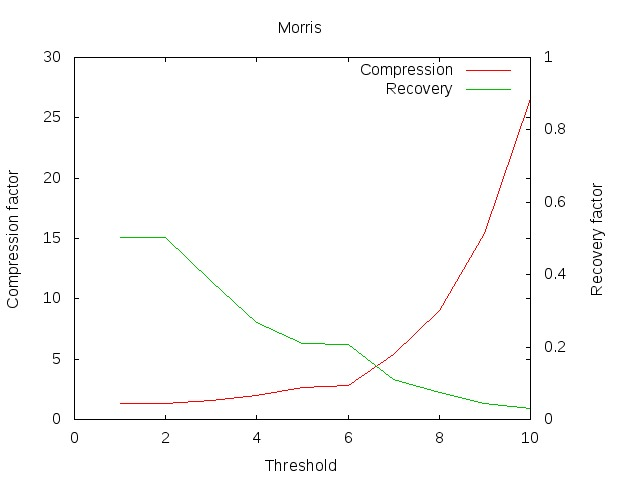
\includegraphics[width=7cm]{images/Morris77.jpg}\hspace{0.5cm}
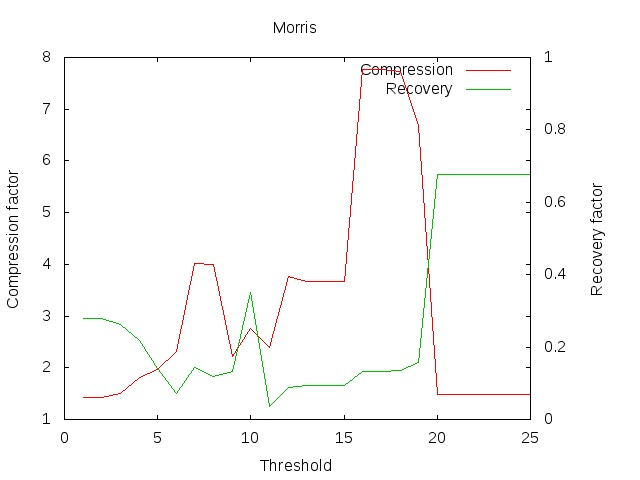
\includegraphics[width=7cm]{images/MorrisDiag.jpg}
\caption{Results with Morris' measure (left: LZ77, right: diagonal patterns)\label{morris}}
\end{figure}

\begin{figure}[h!]
\centering
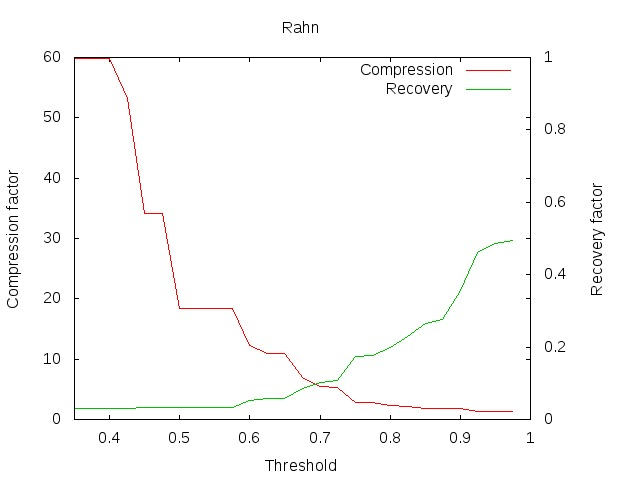
\includegraphics[width=7cm]{images/Rahn77.jpg}\hspace{0.5cm}
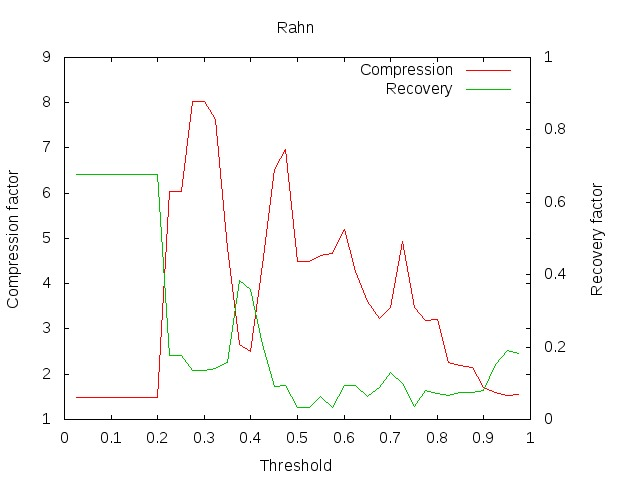
\includegraphics[width=7cm]{images/RahnDiag.jpg}
\caption{Results with Rahn's measure (left: LZ77, right: diagonal patterns)\label{rahn}}
\end{figure}

\begin{figure}[h!]
\centering
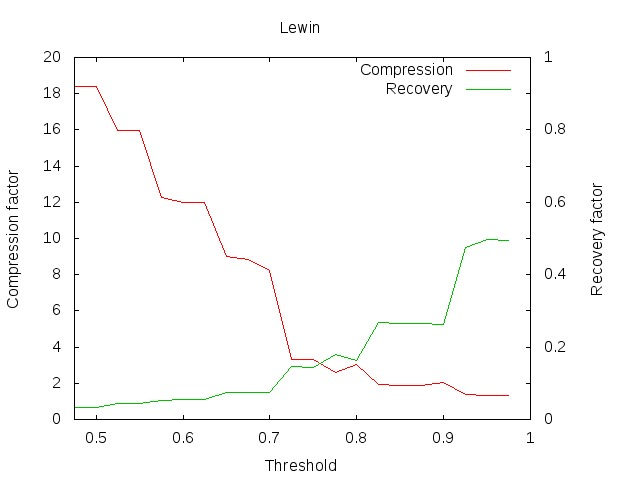
\includegraphics[width=7cm]{images/Lewin77.jpg}\hspace{0.5cm}
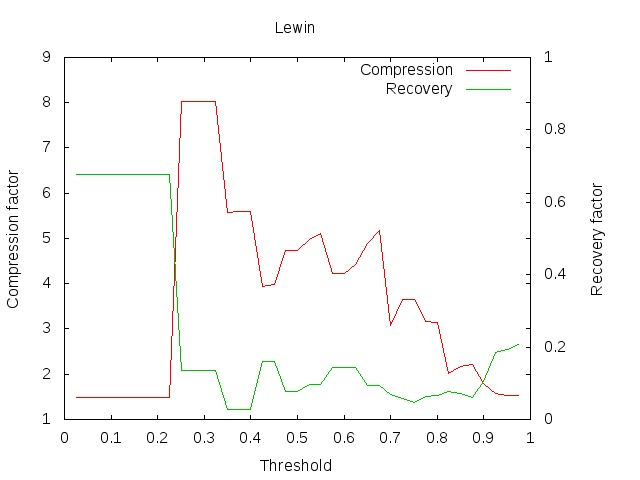
\includegraphics[width=7cm]{images/LewinDiag.jpg}
\caption{Results with Lewin's measure (left: LZ77, right: diagonal patterns)\label{lewin}}
\end{figure}

\begin{figure}[h!]
\centering
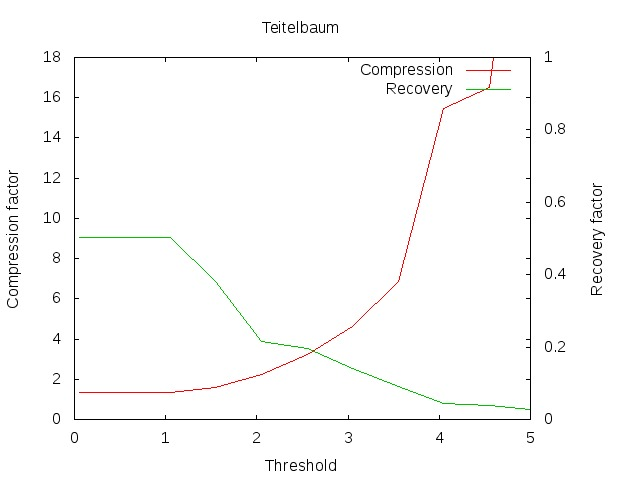
\includegraphics[width=7cm]{images/Teitelbaum77.jpg}\hspace{0.5cm}
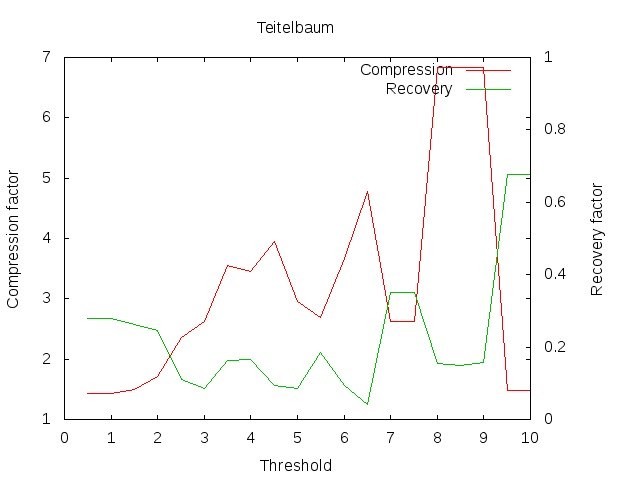
\includegraphics[width=7cm]{images/TeitelbaumDiag.jpg}
\caption{Results with Teitelbaum' measure (left: LZ77, right: diagonal patterns)\label{teitelbaum}}
\end{figure}

\begin{figure}[h!]
\centering
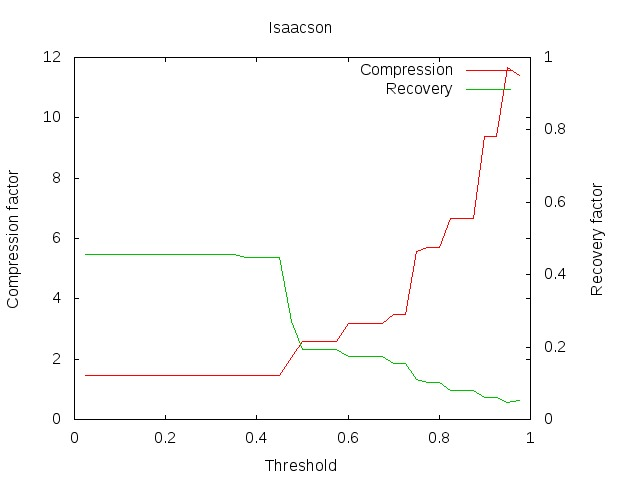
\includegraphics[width=7cm]{images/Isaacson77.jpg}\hspace{0.5cm}
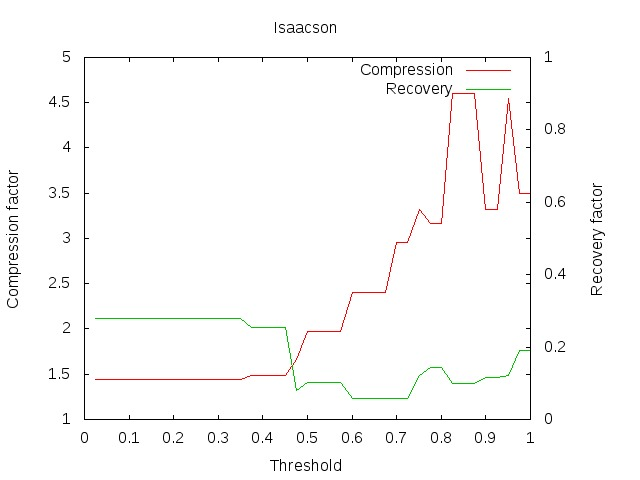
\includegraphics[width=7cm]{images/IsaacsonDiag.jpg}
\caption{Results with Isaacson' measure (left: LZ77, right: diagonal patterns)\label{isaacson}}
\end{figure}

\clearpage

\section{Implementation details}

This section contains some comments on the coding part of the internship.

I have implemented all the algorithms I mention --be it only because I had no other way to evaluate and improve them than watching the results they produced on the data. I coded in C++, a language that I master and that was adapted to the needs of my experiences, since it is fast and that I did not need to perform particularly complex algorithmic operations.

All my code is stored on a GitHub repository, which also contains the data and the numerical results: \href{https://github.com/Rometach/aalborg}{https://github.com/Rometach/aalborg}.


%\section{Institutional context}


%\section{Bibliography}
%\nocite{*}
%
%\bibliographystyle{plain}
%\bibliography{mabiblio}




\end{document}








